\section{Architectures, Adaptation \& Production}

\subsection*{Q: How do Transformers differ from traditional Seq2Seq models?}
\begin{center}
	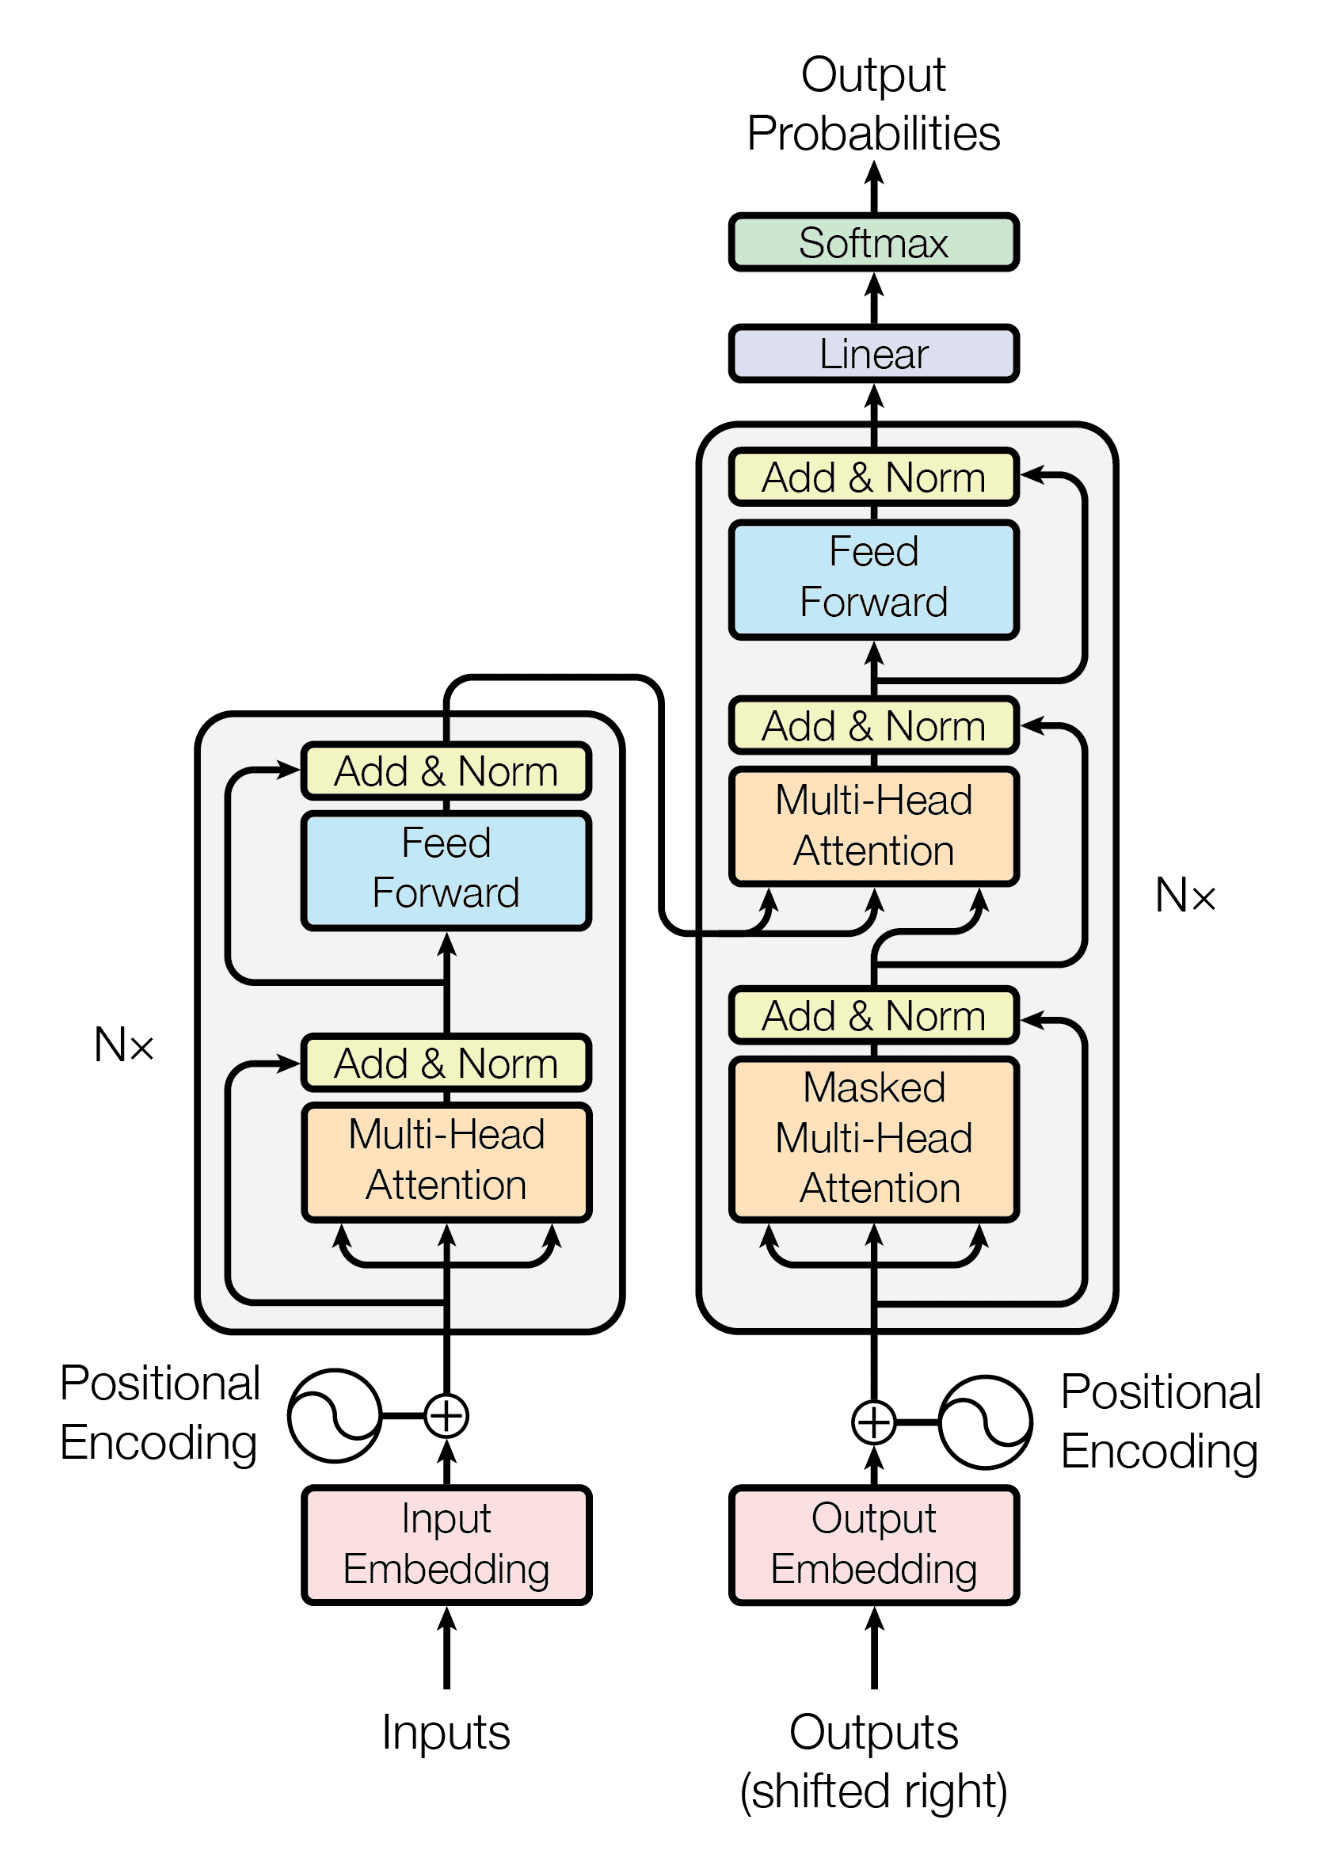
\includegraphics[width=0.4\textwidth]{images/transformer_architecture.png}
\end{center}

\textbf{Transformers} use self-attention instead of recurrence, enabling parallelism and better modeling of long-range dependencies by self-attention and positional embeddings.

Traditional Seq2Seq models (like LSTM-based) process sequences sequentially, making them:
\begin{itemize}
	\item \textbf{Sequential}: Cannot parallelize training across sequence length
	\item \textbf{Memory-limited}: Struggle with very long sequences due to vanishing gradients
	\item \textbf{Position-dependent}: Rely on hidden state to encode position information
\end{itemize}

Transformers address these limitations through:
\begin{itemize}
	\item \textbf{Parallel attention}: All positions can attend to all other positions simultaneously
	\item \textbf{Global receptive field}: Each position can directly access any other position
	\item \textbf{Positional encoding}: Explicit position information through sinusoidal embeddings
\end{itemize}

\subsection*{Q: What are positional embeddings and why are they used in Transformers?}
\textbf{Positional embeddings} encode token positions, which allows the transformer to maintain sequence order since self-attention lacks inherently order awareness, otherwise.

There are two main types of positional embeddings: Absolute and Relative.

Absolute positional embedding, such as learned or sinusoidal positional embedding, uses a fixed positionnal embedding for each token. However, it suffers from the limited sequence length and the independence of positional embeddings.

Relative positional embedding, such as RoPE, uses the relative distance between two positions to encode the positional information, enhancing the model's ability to understanding the relationship among tokens.

Mathematical formulation:
\textbf{Sinusoidal positional embedding}: Uses sinusoidal functions:
\[
	PE_{(pos, 2i)} = \sin\left(\frac{pos}{10000^{2i/d_{\text{model}}}}\right)
\]
\[
	PE_{(pos, 2i+1)} = \cos\left(\frac{pos}{10000^{2i/d_{\text{model}}}}\right)
\]

where \(pos\) is the position and \(i\) is the dimension.

On the other hand, \textbf{Rotary Positional Embedding (RoPE)} uses rotation mechanism to represent each token's position by a rotation in the embedding space:
\[
	\text{RoPE}(x_m, m) = x_m \cos(m\theta) + x_m^{\perp} \sin(m\theta)
\]
where \(\theta\) is a learned parameter and \(x_m^{\perp}\) is a rotated version of \(x_m\).


\subsection*{Q: How do Transformers use positional embeddings in practice?}
\textbf{Positional embeddings} are crucial for transformers to understand sequence order. Here's how they work in practice:

\textbf{1. Integration with Token Embeddings}:
Positional embeddings are added to token embeddings before feeding them into the transformer:
\[
	h_0 = \text{TokenEmbedding}(x) + \text{PositionalEmbedding}(pos)
\]
where \(h_0\) is the input to the first transformer layer, and \(pos\) is the token's position in the sequence.

\textbf{2. Mathematical Properties of Sinusoidal PE}:
The sinusoidal positional encoding has several key properties:

\textbf{Relative Position Learning}:
The model can learn relative positions through trigonometric identities:
\[
	PE_{(pos+k, 2i)} = PE_{(pos, 2i)} \cos\left(\frac{k}{10000^{2i/d_{\text{model}}}}\right) + PE_{(pos, 2i+1)} \sin\left(\frac{k}{10000^{2i/d_{\text{model}}}}\right)
\]

This allows the model to understand that "word at position 5" is 3 positions away from "word at position 2".

\textbf{3. How Self-Attention Uses Positional Information}:
When computing attention scores, the model can learn position-aware patterns:
\[
	\text{Attention}(Q, K, V) = \text{softmax}\left(\frac{(Q + PE_Q)(K + PE_K)^T}{\sqrt{d_k}}\right)(V + PE_V)
\]

The positional embeddings influence attention weights, allowing the model to learn:
\begin{itemize}
	\item \textbf{Local attention}: Nearby tokens often have higher attention scores
	\item \textbf{Positional patterns}: Certain positions may be more important for specific tasks
	\item \textbf{Sequential dependencies}: Order-dependent relationships between tokens
\end{itemize}

\textbf{4. Practical Implementation Details}:

\textbf{Maximum Sequence Length}:
Transformers have a maximum sequence length they can handle:
\begin{itemize}
	\item \textbf{Training}: Usually 512, 1024, or 2048 tokens
	\item \textbf{Inference}: Can extend beyond training length with some methods
	\item \textbf{Memory constraints}: Longer sequences require more memory for attention matrices
\end{itemize}

\textbf{Handling Variable Lengths}:
\begin{itemize}
	\item \textbf{Padding}: Shorter sequences are padded with special tokens
	\item \textbf{Truncation}: Longer sequences are truncated to maximum length
	\item \textbf{Chunking}: Very long sequences can be processed in chunks
\end{itemize}

\textbf{5. Alternative Positional Encoding Methods}:

\textbf{Learned Positional Embeddings}:
\[
	PE_{pos} = W_{pos} \in \mathbb{R}^{d_{\text{model}}}
\]
where \(W_{pos}\) is a learnable parameter for each position.

\textbf{Pros and Cons}:
\begin{itemize}
	\item \textbf{Pros}: Can learn optimal position representations for specific tasks
	\item \textbf{Cons}: Fixed maximum length, doesn't generalize to longer sequences
\end{itemize}

\textbf{Rotary Position Embedding (RoPE)}:
Applies rotation matrices to token embeddings based on position:
\[
	\text{RoPE}(x_m, m) = x_m \cos(m\theta) + x_m^{\perp} \sin(m\theta)
\]
where \(\theta\) is a learned parameter and \(x_m^{\perp}\) is a rotated version of \(x_m\).

\textbf{ALiBi (Attention with Linear Biases)}:
Adds learned bias terms to attention scores:
\[
	\text{Attention}(Q, K, V) = \text{softmax}\left(\frac{QK^T}{\sqrt{d_k}} + B\right)V
\]
where \(B_{ij} = -m|i-j|\) and \(m\) is a learned slope parameter.

\textbf{6. Why Positional Embeddings Matter}:

\textbf{Without Positional Embeddings}:
\begin{itemize}
	\item The sentence "I love you" would be equivalent to "you love I"
	\item Self-attention would treat all positions identically
	\item The model couldn't learn sequential patterns
\end{itemize}

\textbf{With Positional Embeddings}:
\begin{itemize}
	\item Each position has a unique representation
	\item The model can learn position-dependent patterns
	\item Sequential relationships are preserved
	\item Attention can focus on relevant positions
\end{itemize}

\textbf{7. Real-World Examples}:

\textbf{Language Modeling}:
\begin{itemize}
	\item \textbf{Next word prediction}: Position helps understand context
	\item \textbf{Sentence structure}: Grammar depends on word order
	\item \textbf{Document understanding}: Position indicates document structure
\end{itemize}

\textbf{Machine Translation}:
\begin{itemize}
	\item \textbf{Word order differences}: Languages have different word orders
	\item \textbf{Alignment}: Source and target positions need to be learned
	\item \textbf{Context}: Position helps disambiguate meanings
\end{itemize}

\textbf{8. Challenges and Solutions}:

\textbf{Length Generalization}:
\begin{itemize}
	\item \textbf{Problem}: Models trained on shorter sequences may not generalize to longer ones
	\item \textbf{Solutions}:
	      \begin{itemize}
		      \item Use RoPE or ALiBi for better length generalization
		      \item Train on variable-length sequences
		      \item Use hierarchical positional encodings
	      \end{itemize}
\end{itemize}

\textbf{Memory Efficiency}:
\begin{itemize}
	\item \textbf{Problem}: Long sequences require large attention matrices
	\item \textbf{Solutions}:
	      \begin{itemize}
		      \item Sparse attention patterns
		      \item Linear attention mechanisms
		      \item Chunked processing
	      \end{itemize}
\end{itemize}

\subsection*{Q: How does self-attention work?}
\textbf{Self-attention} is a mechanism that allows models to focus on different parts of the input sequence when processing each element. It's the core innovation behind transformer architectures and enables parallel processing while capturing long-range dependencies.

\textbf{Mathematical Formulation}:
The self-attention mechanism computes attention scores and weighted outputs as follows:

\textbf{1. Linear Transformations}:
For input embeddings \(X \in \mathbb{R}^{n \times d}\), we create three matrices:
\[
	Q = XW_Q, \quad K = XW_K, \quad V = XW_V
\]
where \(W_Q, W_K, W_V \in \mathbb{R}^{d \times d_k}\) are learnable weight matrices, and \(d_k\) is the dimension of the key/query space.

\textbf{2. Attention Scores}:
The attention scores are computed as scaled dot-product attention:
\[
	\text{Attention}(Q, K, V) = \text{softmax}\left(\frac{QK^T}{\sqrt{d_k}}\right)V
\]

The scaling factor \(\frac{1}{\sqrt{d_k}}\) prevents the dot products from growing too large, which would push the softmax into regions with small gradients.

\textbf{3. Detailed Computation}:
For each position \(i\), the output is:
\[
	\text{Output}_i = \sum_{j=1}^{n} \alpha_{ij} V_j
\]
where \(\alpha_{ij}\) is the attention weight from position \(i\) to position \(j\):
\[
	\alpha_{ij} = \frac{\exp\left(\frac{Q_i \cdot K_j^T}{\sqrt{d_k}}\right)}{\sum_{k=1}^{n} \exp\left(\frac{Q_i \cdot K_k^T}{\sqrt{d_k}}\right)}
\]

\textbf{Benefits of Self-Attention}:
\begin{itemize}
	\item \textbf{Parallelization}: All attention computations can be done simultaneously
	\item \textbf{Long-range dependencies}: Can directly connect any two positions
	\item \textbf{Interpretability}: Attention weights show what the model is focusing on
	\item \textbf{Flexibility}: Can learn different types of relationships in different heads
\end{itemize}

\subsection*{Q: What are the roles of Query, Key, and Value in self-attention?}

\textbf{Query (Q)} represents "what I'm looking for"; each query learns what information is needed for the current position.
\textbf{Key (K)} represents "what I can offer"; each key learns how to represent its position's content.
\textbf{Value (V)} represents "the actual information"; each value learns to represent information in a way that's useful for downstream tasks.

\textbf{Why Three Separate Representations?}:
\begin{itemize}
	\item \textbf{Separation of concerns}: Query determines what to look for, Key determines relevance, Value provides the content
	\item \textbf{Flexibility}: Different weight matrices allow learning different aspects of the input
	\item \textbf{Interpretability}: Each representation can be analyzed separately to understand model behavior
	\item \textbf{Multi-head attention}: Allows different heads to focus on different types of relationships
\end{itemize}

\subsection*{Q: What is multi-head attention?}

\textbf{Multi-Head Attention}:
Multi-head attention allows the model to attend to different subspaces simultaneously:
\[
	\text{MultiHead}(Q, K, V) = \text{Concat}(\text{head}_1, \ldots, \text{head}_h)W^O
\]
where each head computes:
\[
	\text{head}_i = \text{Attention}(QW_i^Q, KW_i^K, VW_i^V)
\]

\textbf{Benefits of Multi-Head Attention}:
\begin{itemize}
	\item \textbf{Parallel Processing}: Multiple heads compute different relationships simultaneously
	\item \textbf{Specialized Focus}: Each head learns different aspects (syntactic, semantic, positional, task-specific)
	\item \textbf{Ensemble Effect}: Multiple perspectives provide robust understanding
	\item \textbf{Subspace Diversity}: Each head operates in different learned subspaces
	\item \textbf{Regularization}: Prevents overfitting to single attention patterns
	\item \textbf{Interpretability}: Can analyze what each head attends to, enabling debugging and feature visualization
\end{itemize}

\textbf{Computational Complexity}:
\begin{itemize}
	\item \textbf{Time Complexity}: \(O(n^2 \cdot d)\) where \(n\) is sequence length, \(d\) is embedding dimension
	\item \textbf{Space Complexity}: \(O(n^2)\) for storing attention matrices
\end{itemize}

\subsection*{Q: What is Byte Pair Encoding (BPE) and why is it used?}
\textbf{Byte Pair Encoding (BPE)} is a subword tokenization algorithm that decomposes text into units that strike a balance between individual characters and complete words. It begins by treating each character as a separate token and then iteratively merges the most frequent adjacent pairs of tokens into new combined tokens. This approach improves model performance by:
\begin{itemize}
	\item reducing the overall vocabulary size
	\item handling out-of-vocabulary words effectively
	\item improving tokenization efficiency
\end{itemize}

BPE is widely used in modern language models such as GPT and RoBERTa due to its ability to efficiently tokenize large corpora while preserving useful linguistic structures.

The algorithm works as follows:
\begin{enumerate}
	\item Initialize vocabulary with individual characters
	\item Count frequency of adjacent token pairs in training data
	\item Merge most frequent pair into new token
	\item Add new token to vocabulary
	\item Repeat until desired vocabulary size is reached
\end{enumerate}

\textbf{Tokenization process}:
\[
	\text{Tokenize}(text) = \arg\min_{t_1, \ldots, t_n} \sum_{i=1}^{n} \text{Count}(t_i)
\]
where \(t_i\) are subword tokens and \(\text{Count}(t_i)\) is the frequency of token \(t_i\).

\subsection*{Q: What are the common decoding techniques used in large language models (LLMs)?}
Several decoding techniques are used to generate text from large language models, each with different trade-offs between determinism, diversity, and coherence:

\begin{itemize}
	\item \textbf{Greedy Decoding}: This method selects the token with the highest probability at each step. While it is fast and deterministic, it often produces repetitive or suboptimal outputs because it doesn't explore alternative paths.
	\item \textbf{Beam Search}: Beam search keeps track of the top \(k\) most probable sequences (beams) at each decoding step and expands them in parallel. At the end the best sequence with the highest probability is selected. It balances quality and computation by considering multiple candidates, but it can still produce generic responses and is less diverse than sampling-based methods.
	\item \textbf{Top-\(k\) Sampling}: Instead of always choosing the most likely token, top-\(k\) sampling samples a token from the top \(k\) most probable next tokens. This introduces randomness and improves diversity, making outputs more creative and less deterministic.
	\item \textbf{Top-\(p\) Sampling (Nucleus Sampling)}: This method selects a token from the smallest possible set of tokens whose cumulative probability exceeds a threshold \(p\) (e.g., 0.9). It adapts the candidate pool dynamically and often results in more coherent yet diverse outputs compared to top-\(k\) sampling.
	\item \textbf{Temperature Scaling}: Although not a decoding method itself, temperature is a parameter often used during sampling to control randomness. A lower temperature makes the model more confident (peaky distributions), while a higher temperature makes it more random and exploratory.
\end{itemize}

\textbf{Mathematical formulation}:
For top-\(k\) sampling:
\[
	P_{\text{top-k}}(x_i) = \begin{cases}
		\frac{P(x_i)}{\sum_{j \in \text{top-k}} P(x_j)} & \text{if } i \in \text{top-k} \\
		0                                               & \text{otherwise}
	\end{cases}
\]

For top-\(p\) sampling:
\[
	P_{\text{top-p}}(x_i) = \begin{cases}
		\frac{P(x_i)}{\sum_{j \in V_p} P(x_j)} & \text{if } i \in V_p \\
		0                                      & \text{otherwise}
	\end{cases}
\]
where \(V_p\) is the smallest set such that \(\sum_{i \in V_p} P(x_i) \geq p\).

For beam search with beam size \(k\):
\[
	\text{Beam}_t = \arg\max_{S \in \text{Candidates}_t} P(S | x_1, \ldots, x_t)
\]
where \(\text{Candidates}_t\) contains the top \(k\) sequences at step \(t\).

\subsection*{Q: What is MMOE and what are some other multi-objective learning algorithms?}
\begin{itemize}
	\item \textbf{MMOE (Multi-gate Mixture-of-Experts)} is a neural network architecture designed for multi-task learning, where a single model simultaneously learns to perform multiple related tasks. MMOE consists of:
	      \begin{itemize}
		      \item A set of shared \textbf{experts} (typically fully connected networks) that learn general-purpose representations.
		      \item A set of task-specific \textbf{gating networks} that learn how to combine the outputs of the shared experts differently for each task.
	      \end{itemize}
	      This design allows the model to balance shared and task-specific information, improving performance and reducing negative transfer between tasks.

	\item \textbf{Cross-Stitch Networks}: These networks allow linear combinations of activations from task-specific models. The model learns how much information to share at each layer between tasks by learning cross-stitch units.

	\item \textbf{Shared Bottom + Task-Specific Heads}: This is a simple and widely used approach where early layers are shared among tasks to extract common features, while the top layers (heads) are task-specific to capture task-dependent patterns.

	\item \textbf{PLE (Progressive Layered Extraction)}: PLE introduces shared and task-specific experts at multiple levels and progressively separates representations using gating networks, enhancing performance in complex multi-task scenarios.

	\item \textbf{PCGrad (Projected Gradient Descent)}: PCGrad is an optimization-based method for multi-objective learning. It resolves gradient conflicts between tasks by projecting conflicting gradients onto each other's normal planes, avoiding destructive interference during learning.

	\item \textbf{GradNorm}: This algorithm dynamically balances the training of multiple tasks by adjusting the gradients' magnitudes to ensure that all tasks train at a similar rate, preventing task dominance.

\end{itemize}

Multi-objective and multi-task learning algorithms are especially useful when tasks are related and can benefit from shared representations, improving generalization and model efficiency.

\textbf{MMOE mathematical formulation}:
For task \(k\), the output is:
\[
	y_k = \sum_{i=1}^{n} g_k^i(x) \cdot f_i(x)
\]
where \(g_k^i(x)\) is the gating network output for expert \(i\) on task \(k\), and \(f_i(x)\) is the output of expert \(i\).

The gating network uses softmax:
\[
	g_k^i(x) = \frac{\exp(h_k^i(x))}{\sum_{j=1}^{n} \exp(h_k^j(x))}
\]
where \(h_k^i(x)\) is the logit for expert \(i\) on task \(k\).

\subsection*{Q: What are Mixture of Experts (MoE) architectures and how do they work?}
\textbf{Mixture of Experts (MoE)} is a neural architecture that consists of multiple expert networks and a gating network that dynamically routes inputs to the most relevant experts. This approach enables models to scale to very large parameter counts while maintaining computational efficiency through conditional computation.

\textbf{Core components}:
\begin{itemize}
	\item \textbf{Expert Networks}: Specialized sub-networks that learn different aspects of the input space
	\item \textbf{Gating Network}: A router that determines which experts should process each input
	\item \textbf{Combination Mechanism}: Aggregates expert outputs based on gating probabilities
\end{itemize}

\textbf{Mathematical formulation}:
For input \(x\), the MoE output is:
\[
	y = \sum_{i=1}^{n} g_i(x) \cdot f_i(x)
\]
where \(g_i(x)\) is the gating probability for expert \(i\), and \(f_i(x)\) is the output of expert \(i\).

The gating network typically uses softmax:
\[
	g_i(x) = \frac{\exp(h_i(x))}{\sum_{j=1}^{n} \exp(h_j(x))}
\]
where \(h_i(x)\) is the logit for expert \(i\).

\textbf{Key advantages}:
\begin{itemize}
	\item \textbf{Scalability}: Can handle billions of parameters efficiently
	\item \textbf{Specialization}: Experts can specialize in different input patterns
	\item \textbf{Conditional computation}: Only active experts consume compute
	\item \textbf{Modularity}: Easy to add/remove experts or modify routing
\end{itemize}

\subsection*{Q: What are the different types of MoE architectures?}
Several variants of MoE have been developed for different use cases:

\begin{itemize}
	\item \textbf{Traditional MoE}: Basic mixture of experts with soft routing
	\item \textbf{Sparse MoE}: Only activates top-k experts per input (e.g., Switch Transformers)
	\item \textbf{Hierarchical MoE}: Organizes experts in a tree structure
	\item \textbf{Task-specific MoE}: Different expert sets for different tasks
	\item \textbf{Dynamic MoE}: Adapts expert selection based on input characteristics
\end{itemize}

\textbf{Sparse MoE} (most common in practice):
Instead of using all experts, sparse MoE selects the top-k experts:
\[
	g_i(x) = \begin{cases}
		\frac{\exp(h_i(x))}{\sum_{j \in \text{top-k}} \exp(h_j(x))} & \text{if } i \in \text{top-k} \\
		0                                                           & \text{otherwise}
	\end{cases}
\]

This reduces computation from \(O(n)\) to \(O(k)\) where \(k \ll n\).

\textbf{Switch Transformers} use \(k=1\) (single expert per input), making them extremely efficient:
\[
	y = f_{\arg\max_i h_i(x)}(x)
\]

\subsection*{Q: How does routing work in MoE architectures?}
\textbf{Routing} in MoE determines which experts should process each input. The routing mechanism is crucial for both performance and efficiency.

\textbf{Soft routing} (traditional MoE):
\[
	g_i(x) = \text{softmax}(h_i(x))_i
\]
All experts contribute to the output, weighted by their gating probabilities.

\textbf{Hard routing} (sparse MoE):
\[
	g_i(x) = \begin{cases}
		1 & \text{if } i = \arg\max_j h_j(x) \\
		0 & \text{otherwise}
	\end{cases}
\]
Only the most relevant expert contributes to the output.

\textbf{Top-k routing}:
\[
	g_i(x) = \begin{cases}
		\frac{\exp(h_i(x))}{\sum_{j \in \text{top-k}} \exp(h_j(x))} & \text{if } i \in \text{top-k} \\
		0                                                           & \text{otherwise}
	\end{cases}
\]
The top-k experts contribute, weighted by their relative scores.

\textbf{Routing strategies}:
\begin{itemize}
	\item \textbf{Load balancing}: Ensures experts are used evenly across inputs
	\item \textbf{Expert diversity}: Prevents routing collapse to a few experts
	\item \textbf{Noise injection}: Adds randomness to prevent deterministic routing
	\item \textbf{Auxiliary losses}: Additional objectives to improve routing quality
\end{itemize}

\subsection*{Q: What are the challenges and solutions in training MoE models?}
\textbf{Training MoE models} presents several unique challenges:

\textbf{Load balancing}:
\begin{itemize}
	\item \textbf{Problem}: Experts may receive very few inputs, leading to poor training
	\item \textbf{Solutions}:
	      \begin{itemize}
		      \item Auxiliary load balancing loss
		      \item Expert diversity regularization
		      \item Noise injection in routing
		      \item Expert dropout during training
	      \end{itemize}
\end{itemize}

\textbf{Routing collapse}:
\begin{itemize}
	\item \textbf{Problem}: Gating network may always select the same experts
	\item \textbf{Solutions}:
	      \begin{itemize}
		      \item Entropy regularization on gating distribution
		      \item Expert diversity constraints
		      \item Curriculum learning for routing
	      \end{itemize}
\end{itemize}

\textbf{Gradient flow}:
\begin{itemize}
	\item \textbf{Problem}: Gradients may not flow well through the routing mechanism
	\item \textbf{Solutions}:
	      \begin{itemize}
		      \item Straight-through estimators
		      \item Gumbel-softmax for differentiable routing
		      \item REINFORCE for discrete routing
	      \end{itemize}
\end{itemize}

\textbf{Mathematical formulations}:

\textbf{Load balancing loss}:
\[
	\mathcal{L}_{\text{load}} = \alpha \sum_{i=1}^{n} \left(\frac{1}{B} \sum_{b=1}^{B} g_i(x_b) - \frac{1}{n}\right)^2
\]
where \(B\) is batch size and \(\alpha\) controls the strength of load balancing.

\textbf{Expert diversity loss}:
\[
	\mathcal{L}_{\text{diversity}} = \beta \sum_{i \neq j} \text{sim}(f_i, f_j)
\]
where \(\text{sim}(f_i, f_j)\) measures similarity between expert outputs.

\subsection*{Q: How do MoE architectures scale to large models?}
\textbf{MoE scaling} enables training of extremely large models efficiently:

\textbf{Parameter scaling}:
\begin{itemize}
	\item \textbf{Expert parameters}: Can scale to billions of parameters per expert
	\item \textbf{Shared parameters}: Routing and other components remain constant
	\item \textbf{Total parameters}: Can reach trillions of parameters
\end{itemize}

\textbf{Computational scaling}:
\begin{itemize}
	\item \textbf{Per-token computation}: Only active experts consume compute
	\item \textbf{Memory efficiency}: Experts can be distributed across devices
	\item \textbf{Inference speed}: Scales with number of active experts, not total experts
\end{itemize}

\textbf{Distributed training strategies}:
\begin{itemize}
	\item \textbf{Expert parallelism}: Distribute experts across multiple devices
	\item \textbf{Data parallelism}: Replicate experts across devices
	\item \textbf{Hybrid approaches}: Combine both strategies for optimal scaling
\end{itemize}

\textbf{Mathematical analysis}:
For a model with \(n\) experts, each with \(p\) parameters:
\begin{itemize}
	\item \textbf{Total parameters}: \(O(n \cdot p)\)
	\item \textbf{Active parameters per input}: \(O(k \cdot p)\) where \(k\) is routing sparsity
	\item \textbf{Computation ratio}: \(\frac{k}{n}\) (e.g., 1/8 for top-1 routing with 8 experts)
\end{itemize}

\textbf{Memory considerations}:
\begin{itemize}
	\item \textbf{Expert memory}: \(O(n \cdot p)\) parameters stored
	\item \textbf{Activation memory}: \(O(k \cdot p)\) activations computed
	\item \textbf{Routing memory}: \(O(n)\) gating probabilities
\end{itemize}

\subsection*{Q: What are the applications and use cases for MoE architectures?}
\textbf{MoE architectures} have found success in various domains:

\textbf{Natural Language Processing}:
\begin{itemize}
	\item \textbf{Large language models}: GPT-4, PaLM, Switch Transformers
	\item \textbf{Machine translation}: Multi-lingual models with language-specific experts
	\item \textbf{Text generation}: Domain-specific experts for different writing styles
\end{itemize}

\textbf{Computer Vision}:
\begin{itemize}
	\item \textbf{Image classification}: Experts for different visual patterns
	\item \textbf{Object detection}: Experts for different object categories
	\item \textbf{Multi-modal tasks}: Separate experts for different input modalities
\end{itemize}

\textbf{Recommendation Systems}:
\begin{itemize}
	\item \textbf{User modeling}: Experts for different user segments
	\item \textbf{Content understanding}: Experts for different content types
	\item \textbf{Multi-objective optimization}: Balancing multiple objectives
\end{itemize}

\textbf{Multi-task Learning}:
\begin{itemize}
	\item \textbf{Task-specific experts}: Specialized experts for different tasks
	\item \textbf{Shared representations}: Common experts for shared knowledge
	\item \textbf{Transfer learning}: Leveraging expertise across related tasks
\end{itemize}

\textbf{Key benefits in these applications}:
\begin{itemize}
	\item \textbf{Scalability}: Handle larger models and datasets
	\item \textbf{Specialization}: Experts can focus on specific patterns
	\item \textbf{Efficiency}: Conditional computation reduces resource usage
	\item \textbf{Flexibility}: Easy to adapt to new tasks or domains
\end{itemize}

\subsection*{Q: What is PEFT (Parameter-Efficient Fine-Tuning)?}
\textbf{PEFT} fine-tunes only a subset of parameters, reducing memory and compute costs while preserving performance.

PEFT methods include:
\begin{itemize}
	\item \textbf{LoRA (Low-Rank Adaptation)}: Adds low-rank trainable matrices to frozen layers
	\item \textbf{Adapter Layers}: Inserts small trainable layers between frozen layers
	\item \textbf{Prefix Tuning}: Prepends trainable prefix tokens to input
	\item \textbf{Prompt Tuning}: Trains continuous prompt embeddings
	\item \textbf{BitFit}: Only fine-tunes bias terms
\end{itemize}

\textbf{Benefits}:
\begin{itemize}
	\item Reduced memory footprint (can fine-tune large models on consumer hardware)
	\item Faster training and inference
	\item Better preservation of pre-trained knowledge
	\item Easier model sharing and deployment
\end{itemize}

\subsection*{Q: What is LoRA and how does it work?}
\textbf{LoRA} adds low-rank trainable matrices to frozen layers, reducing the number of trainable parameters for speed and memory-efficiency.

For a pre-trained weight matrix \(W_0 \in \mathbb{R}^{d \times k}\), LoRA parameterizes its change during adaptation as:
\[
	W = W_0 + \Delta W = W_0 + BA
\]
where \(B \in \mathbb{R}^{d \times r}\) and \(A \in \mathbb{R}^{r \times k}\) are low-rank matrices with rank \(r \ll \min(d, k)\).

The forward pass becomes:
\[
	h = Wx = W_0x + \Delta Wx = W_0x + BAx
\]

\textbf{Key advantages}:
\begin{itemize}
	\item \textbf{Memory efficient}: Only stores \(B\) and \(A\) instead of full \(\Delta W\)
	\item \textbf{Fast adaptation}: Low-rank structure allows efficient updates
	\item \textbf{Modular}: Can easily switch between different LoRA adapters
	\item \textbf{Composable}: Multiple LoRA adapters can be combined
\end{itemize}

\textbf{Optimal rank selection}:
The rank \(r\) is a hyperparameter that balances:
\begin{itemize}
	\item \textbf{Expressiveness}: Higher rank allows more complex adaptations
	\item \textbf{Efficiency}: Lower rank reduces memory and computation
	\item \textbf{Generalization}: Lower rank can prevent overfitting
\end{itemize}

\subsection*{Q: What is QLoRA and why is it useful?}
\textbf{QLoRA} applies LoRA to the quantized models (e.g., 4-bit), enabling fine-tuning of large models on limited hardware. Once all the training is done, the original weights will be de-quantized.

QLoRA uses 4-bit NormalFloat (NF4) quantization, which:
\begin{itemize}
	\item Reduces memory usage by 8x compared to 16-bit precision
	\item Maintains model performance through careful quantization
	\item Enables fine-tuning of 65B+ parameter models on consumer hardware
\end{itemize}

\textbf{Quantization process}:
For a weight matrix \(W\), NF4 quantization:
\begin{enumerate}
	\item Normalizes weights to \([-1, 1]\) range
	\item Maps to 16 discrete values using normal distribution
	\item Stores only 4 bits per weight
\end{enumerate}

\textbf{Memory savings}:
\begin{itemize}
	\item \textbf{Model weights}: 4-bit instead of 16-bit (4x reduction)
	\item \textbf{LoRA adapters}: Only train low-rank matrices
	\item \textbf{Total memory}: 8-16x reduction compared to full fine-tuning
\end{itemize}

\subsection*{Q: What is collaborative filtering and what are its types?}
\textbf{Collaborative filtering} recommends items based on user/item similarity. Types include user-based, item-based, and matrix factorization.

\textbf{User-based CF} finds similar users and recommends items they liked:
\[
	\text{sim}(u, v) = \frac{\sum_{i \in I_{uv}} (r_{ui} - \bar{r}_u)(r_{vi} - \bar{r}_v)}{\sqrt{\sum_{i \in I_{uv}} (r_{ui} - \bar{r}_u)^2} \sqrt{\sum_{i \in I_{uv}} (r_{vi} - \bar{r}_v)^2}}
\]
where \(r_{ui}\) is user \(u\)'s rating for item \(i\), and \(I_{uv}\) is the set of items rated by both users.

\textbf{Item-based CF} finds similar items and recommends them:
\[
	\text{sim}(i, j) = \frac{\sum_{u \in U_{ij}} (r_{ui} - \bar{r}_i)(r_{uj} - \bar{r}_j)}{\sqrt{\sum_{u \in U_{ij}} (r_{ui} - \bar{r}_i)^2} \sqrt{\sum_{u \in U_{ij}} (r_{uj} - \bar{r}_j)^2}}
\]

\textbf{Matrix Factorization} decomposes the rating matrix \(R \in \mathbb{R}^{m \times n}\) into:
\[
	R \approx UV^T
\]
where \(U \in \mathbb{R}^{m \times k}\) and \(V \in \mathbb{R}^{n \times k}\) are user and item latent factor matrices.

The objective function is:
\[
	\min_{U, V} \sum_{(u,i) \in \Omega} (r_{ui} - u_u^T v_i)^2 + \lambda(\|U\|_F^2 + \|V\|_F^2)
\]
where \(\Omega\) is the set of observed ratings and \(\lambda\) is the regularization parameter.

\subsection*{Q: What are the limitations of collaborative filtering?}
\begin{itemize}
	\item \textbf{Cold-start problem}: Collaborative filtering requires a history of user-item interactions to make recommendations. When new users or items enter the system, the lack of historical data makes it difficult to generate accurate recommendations.
	\item \textbf{Data sparsity}: In many real-world applications, users interact with only a small fraction of available items, leading to a sparse user-item matrix. This sparsity reduces the effectiveness of similarity-based methods and can negatively impact the quality of recommendations.
	\item \textbf{Scalability}: As the number of users and items grows, computing similarity scores and performing matrix factorization becomes computationally expensive, posing challenges for real-time recommendation at scale.
	\item \textbf{Popularity bias}: Collaborative filtering tends to recommend popular items more frequently, which can lead to a lack of diversity in recommendations and overlook niche or less-rated content.
	\item \textbf{Lack of contextual understanding}: Collaborative filtering does not typically incorporate side information such as time, location, or user demographics, which may be crucial for making context-aware recommendations.
\end{itemize}

\subsection*{Q: What is the two-tower model?}
The \textbf{two-tower model} is a neural architecture commonly used for tasks like recommendation, retrieval, and matching. It consists of two separate neural networks (or "towers")—one for encoding the query (e.g., user, question, search term) and one for encoding the candidate (e.g., item, product, document). Each tower processes its input independently to produce dense vector embeddings.

The similarity between the query and candidate embeddings is then computed—typically using dot product or cosine similarity—to rank or retrieve relevant items. This architecture is efficient for large-scale retrieval since it allows for precomputing and indexing embeddings, enabling fast approximate nearest neighbor (ANN) search.

Key advantages include:
\begin{itemize}
	\item Decoupled processing of queries and items, allowing independent optimization.
	\item Scalability due to efficient embedding retrieval via vector similarity.
	\item Simplicity and interpretability of embedding space.
\end{itemize}

Limitations include:
\begin{itemize}
	\item No cross-interaction between query and item features during encoding.
	\item Suboptimal performance in tasks where joint modeling is important.
\end{itemize}

\subsection*{Q: What are the newer model architectures beyond the two-tower model?}
Several newer architectures have been proposed to address the limitations of the two-tower model, particularly to capture richer interactions between queries and candidates:

\begin{itemize}
	\item \textbf{Cross-Encoder}: Instead of encoding query and candidate separately, a cross-encoder concatenates both inputs and feeds them into a single transformer (e.g., BERT). This allows for deep interaction between inputs and often achieves higher accuracy—but at a much higher computational cost, making it unsuitable for large-scale retrieval.

	\item \textbf{Poly-Encoder}: Proposed by Facebook AI, the poly-encoder balances efficiency and interaction. It uses multiple context vectors (instead of a single one) to attend over the candidate representations. It achieves a middle ground between two-tower and cross-encoder models in terms of performance and speed.

	\item \textbf{ColBERT (Contextualized Late Interaction)}: ColBERT introduces late interaction by computing token-level embeddings using BERT and applying a MaxSim operation across tokens. This allows fine-grained matching while still supporting fast retrieval through ANN techniques.

	\item \textbf{Retriever-Ranker Architecture}: This hybrid approach first uses a fast two-tower retriever to narrow down candidates and then applies a more expressive cross-encoder to re-rank the top candidates. It is widely used in large-scale systems like search engines and QA pipelines.

	\item \textbf{Dense-Sparse Hybrid Models}: Some models combine dense retrieval (like two-tower or ColBERT) with sparse representations (e.g., TF-IDF or BM25) to leverage both semantic similarity and lexical overlap.
\end{itemize}

These newer models improve retrieval accuracy by modeling cross-input interactions, at the cost of increased inference latency and system complexity.

\textbf{Performance comparison}:
\begin{itemize}
	\item \textbf{Two-Tower}: Fastest inference, lowest accuracy
	\item \textbf{Poly-Encoder}: Medium speed, medium accuracy
	\item \textbf{Cross-Encoder}: Slowest inference, highest accuracy
	\item \textbf{Hybrid}: Balanced approach with retriever + reranker
\end{itemize}

The choice depends on the trade-off between accuracy and latency requirements in your specific use case.

\subsection*{Q: What is multi-task learning (MTL) and why is it useful?}
\textbf{Multi-task learning (MTL)} is a machine learning paradigm where a single model learns to perform multiple related tasks simultaneously. Instead of training separate models for each task, MTL leverages shared representations and knowledge transfer to improve performance across all tasks.

\textbf{Key Benefits}:
\begin{itemize}
	\item \textbf{Improved Generalization}: Shared representations help prevent overfitting and improve generalization
	\item \textbf{Knowledge Transfer}: Knowledge learned for one task can benefit other related tasks
	\item \textbf{Reduced Computational Cost}: Single model instead of multiple specialized models
	\item \textbf{Better Feature Learning}: Shared layers can learn more robust and generalizable features
	\item \textbf{Regularization Effect}: Multi-task objectives act as implicit regularization
\end{itemize}

\textbf{Challenges}:
\begin{itemize}
	\item \textbf{Task Balancing}: Different tasks may have different scales or importance
	\item \textbf{Negative Transfer}: Some tasks may interfere with each other
	\item \textbf{Architecture Design}: Finding the right balance between shared and task-specific components
	\item \textbf{Training Stability}: Managing gradients from multiple objectives
\end{itemize}

\subsection*{Q: What commonly goes wrong with the classic shared-bottom MTL?}
\textbf{Negative transfer} occurs when tasks with weak or anti-correlation interfere with each other. Improvements in one head can hurt another, creating a \emph{seesaw effect} where overall performance doesn't improve despite individual task gains.

Flat sharing often \emph{does not scale} as you add more tasks or increase task heterogeneity (e.g., short-term clicks vs. long-term value prediction). This motivates the need for more sophisticated sharing mechanisms.

\subsection*{Q: Which static sharing baselines would you try before expert routing?}
\textbf{Cross-stitch / Sluice} networks learn what to share versus what to keep separate between task towers. These provide strong baselines and are easy to reason about, making them excellent starting points before implementing more complex expert routing approaches.

\subsection*{Q: How do Mixture-of-Experts (MoE) and MMoE help in recommendation MTL?}
MoE and MMoE replace a single shared trunk with multiple \emph{experts}. Each task has a \textbf{gate} that softly routes inputs to experts, enabling input- and task-conditional sharing.

For task $k$, the gate $g^{(k)}(x)=\mathrm{softmax}(W^{(k)}x)$ combines expert outputs $\{f_i(x)\}$ into $z^{(k)}=\sum_i g^{(k)}_i(x) f_i(x)$. Then a task-specific tower $q^{(k)}(z^{(k)})$ outputs the final prediction $\hat y_k$.

\textbf{Key differences}: MoE uses a single gating network for all tasks, while MMoE uses task-specific gates $g^{(k)}(x)$ for each task $k$. This allows MMoE to learn task-specific routing patterns.

Benefits include reduced interference between tasks, adaptive sharing by user/item segment (e.g., new users/items), and the ability to scale without exploding the model count.

\subsection*{Q: What does PLE (Progressive Layered Extraction) add beyond MMoE?}
PLE explicitly separates \textbf{shared experts} and \textbf{task-specific experts} and \emph{stacks} them in layers. Each layer's gates draw from both pools, creating a hierarchical structure.

\textbf{Progressive mechanism}: At each layer $l$, the model computes $z^{(k)}_l = \sum_i g^{(k)}_{l,i}(x) f_{l,i}(x)$, where experts $f_{l,i}$ can be either shared or task-specific. Lower layers focus on shared representations, while higher layers progressively extract task-specific features.

This approach progressively refines shared semantics at lower layers and specialization at higher layers, effectively mitigating seesaw effects as the number of tasks proliferates. PLE represents an evolution beyond MMoE by introducing explicit layering and progressive extraction.

\subsection*{Q: How do you handle label imbalance and conflicting objectives?}
Use per-task losses (BCE for binary heads, MSE for regressions) with \textbf{task weights} or advanced techniques like GradNorm/uncertainty weighting. Consider focal loss for extreme imbalance scenarios.

\textbf{Task weighting strategies}:
\begin{itemize}
	\item \textbf{Static weights}: Manually set based on business priorities
	\item \textbf{Dynamic weights}: Learn weights during training (e.g., GradNorm)
	\item \textbf{Uncertainty weighting}: Weight by task uncertainty estimates
\end{itemize}

Down/upsample by task or apply temperature-scaled soft-parameters in fusion to avoid over-optimizing easy but less valuable heads. This ensures balanced training across all objectives.
